\documentclass[11pt]{article}
\usepackage[T1]{fontenc}
\usepackage{amsmath,newtxtext,newtxmath}
\usepackage{microtype,booktabs,array,graphicx}
\usepackage[margin=1in]{geometry}
\usepackage[font=small,labelfont=bf]{caption}
\usepackage[hidelinks]{hyperref}
\usepackage{xurl}
\hypersetup{pdftitle={DraftFM After Release: First Picks in The Hobbit and a Preview of Reality Fracture},pdfauthor={Brian Ward}}
\setlength{\emergencystretch}{3em}
\setlength{\textfloatsep}{14pt}
\renewcommand{\topfraction}{0.9}
\renewcommand{\bottomfraction}{0.8}
\renewcommand{\textfraction}{0.08}
\widowpenalty=10000
\clubpenalty=10000
\newcommand{\datadir}{data/followup_20260920}
\newcommand{\code}[1]{\texttt{\detokenize{#1}}}

\title{DraftFM After Release:\\First Picks in \emph{The Hobbit} and a Preview of \emph{Reality Fracture}}
\author{Brian Ward\\{\small Independent Researcher}}
\date{September 25, 2026 --- Working draft}

\begin{document}
\maketitle
\begin{abstract}
The original DraftFM paper promised an evaluation of its prerelease
\emph{The Hobbit} (HOB) forecast once human drafts became available. This note
reports that evaluation. On 6,493 opening packs from experienced winning
players, the sealed ranking agrees with 47.34\% of first picks, compared with
54.33\% for the archived Limited Level-Ups review. DraftFM's differences from
Nizzahon and NicolaiBolas are unresolved by paired intervals; it leads three
other archived forecasts. Across all 41,093 shared drafts, DraftFM has the
highest agreement among the prerelease comparators. A separate, exploratory
model learning just 188 card values from post-release expert picks reaches
68.15\% in five-fold held-out evaluation. The results support useful transfer
to an unseen set while showing a substantial advantage from observing its
drafts. We explain the scope of first-pick evaluation and how a sealed ranking
can support actual opening-pack recommendations. We then preview the same
frozen model's \emph{Reality Fracture} (FRA) ranking, including its conspicuous
choice of Terminal Criticism as the highest-ranked uncommon. HOB results
measure agreement with choices; FRA predictions remain untested.
\end{abstract}

\section{Following through on a prerelease forecast}

DraftFM was built for the interval between knowing a new set's cards and
having examples of people drafting them. The original paper describes a
model that represents cards through public structured attributes and a fixed
text embedding, then scores available choices using the drafted pool and
draft context~\cite{draftfm}. Its final model was fitted on 32 previously
observed expansions, with no HOB draft examples. The HOB card ranking was
generated on August 9, 2026 and published under the \code{draftfm-v1.0} tag
before the August 11 Arena release~\cite{seal}.

That public artifact gives this follow-up a concrete prediction to test.
We load the original CSV and verify its digest. We do not rerun the model,
choose a newer checkpoint, or revise the ranking using HOB results. The
comparison therefore concerns the forecast readers could have obtained
before release. The detailed analysis rules were written after release but
before calculating the comparison; the forecast is prospective and the
analysis is retrospective. This distinction matters more than calling the
whole exercise a preregistration.

The main question is modest: when a player opens a fresh pack, how often
does the highest-ranked card coincide with the card they take? The answer
can be compared with saved human reviews on the same packs. It cannot by
itself identify the best possible pick, assign a causal win-rate benefit, or
establish how well an assistant manages an entire draft.

\section{A common first-pick task}

\subsection{Why the opening pick is a useful comparison}

At pack one, pick one (P1P1), the drafter has no previously selected cards.
There is no pool color commitment, curve to repair, or accumulated synergy
to favor one card over another. A prerelease card ranking can therefore
make a concrete prediction without inventing a way to turn its grades into
a full drafting policy. Restrict each ranking to the cards actually offered
and take its highest-rated choice.

This also fits the frozen DraftFM architecture. With the empty pool and
skill, format, position, and set inputs fixed, each candidate receives its
own score. The final export has no whole-set context encoder and no
interaction among the offered candidates. Removing alternatives changes
the softmax denominator, but does not change the relative order of two
remaining cards. Consequently, the published set ranking suffices for this
particular first-pick policy. It is not necessary to simulate a draft or
rerun the neural network for every opening pack.

First-pick agreement still measures behavior. Strong players can reasonably
disagree, select for different strategies, or follow reviews they have seen.
The saved reviews and observed players are not necessarily independent
sources of judgment. A reviewer who predicts those choices well has passed
this benchmark; that does not demonstrate superior game outcomes. Later
picks would require pool-conditioned policies for a fair comparison with
the full DraftFM model.

\subsection{Data, coverage, and ties}

The frozen 17Lands Premier Draft file contains 1,833,289 pick rows and
43,650 distinct HOB opening picks, dated August 11--29~\cite{lands}. It was
downloaded on September 19; the download date is not the end of the observed
play period. We use the original paper's experienced-player thresholds:
win-rate bucket at least 0.55 and games-played bucket at least 100. Of the
43,650 drafts, 6,902 satisfy both. This is an operational player slice, not
a claim that every selected action is expert ground truth.

Every predictor in a shared comparison must rate every offered non-basic
card. Limited Level-Ups marked \emph{The Black Arrow} as sideboard-only,
leaving it without a main-deck rank in our transcription. The shared
comparison excludes its 2,557 packs, including 409 experienced-player packs.
The resulting populations contain 41,093 and 6,493 drafts, respectively.
No observed first pick was a basic land or an unknown card. Larger pairwise
comparisons remain available in the accompanying results.

The other archived full-set forecasts are NicolaiBolas, Nizzahon, Card Game
Base, the Draftsim app pick order, and the Draftsim written review. The two
Draftsim forecasts are distinct archived inputs, not two independent
organizations. Limited Resources is present in the archive but covers only
120 commons and uncommons. It has no fully covered opening packs and thus
no comparable row in the main table.

Letter grades retain their ordinal ordering; numeric scores retain their
native values. Slash grades use the first grade under the recorded analysis
rule. For offered non-basic card names $C_d$ in draft $d$, let $T_{m,d}$ be
the set tied for the highest rating from predictor $m$, and let $y_d$ be the
observed pick. The per-draft agreement credit is
\begin{equation}
 a_{m,d}=\frac{\mathbf{1}\{y_d\in T_{m,d}\}}{|T_{m,d}|}.
\end{equation}
This is expected agreement under uniform tie-breaking. It avoids favoring
a source merely because its scale produces more ties. Card names, rather
than duplicate printings of the same card, define the alternatives.

We average credit across the identical eligible drafts for each predictor.
Differences receive paired percentile intervals from 2,000 draft resamples,
with seed 17. There is exactly one P1P1 row per draft. These are marginal
95\% intervals without multiple-comparison adjustment, and draft resampling
does not account for repeated appearances of the same player.

\section{HOB results: useful transfer, with a clear human lead}

Table~\ref{tab:headline} reports both player populations. The
experienced-player slice is primary because it matches the forecast's
intended skill condition. Limited Level-Ups reaches 54.33\% agreement,
compared with DraftFM's 47.34\%. Its 6.99-point advantage has a paired
95\% interval of 5.54--8.38 points: approximately seven additional matching
first picks per hundred packs under the tie-breaking convention. That is a
meaningful lead on this task.

\begin{table}[htbp]
\centering\small
\input{\datadir/headline.tex}
\caption{First-pick agreement on identical packs: 6,493 experienced-player
drafts and 41,093 all-player drafts. The HOB-trained model uses post-release
data with each scored draft held out; it is a separate reference, not a
prerelease forecast. Uniform random chooses among distinct offered non-basic
card names.}\label{tab:headline}
\end{table}

DraftFM's results against the remaining archived forecasts are more
competitive. The paired differences from Nizzahon and NicolaiBolas cross
zero (Table~\ref{tab:paired}). That leaves their ordering unresolved at this
precision; it does not establish equivalence. DraftFM leads Card Game Base
and both Draftsim inputs under the same analysis.

\begin{table}[htbp]
\centering\small
\input{\datadir/paired.tex}
\caption{Paired differences on experienced-player packs, in percentage
points. Positive values favor DraftFM. Intervals condition on the recorded
predictions, including the fitted model's held-out predictions.}
\label{tab:paired}
\end{table}

The all-player column reverses the DraftFM--Limited Level-Ups ordering:
50.61\% against 49.13\%. DraftFM leads all six prerelease comparators there.
Reporting both slices reveals this difference rather than selecting the
population that gives a preferred story. The present analysis does not
isolate why the population changes the ordering.

\begin{figure}[htbp]
\centering
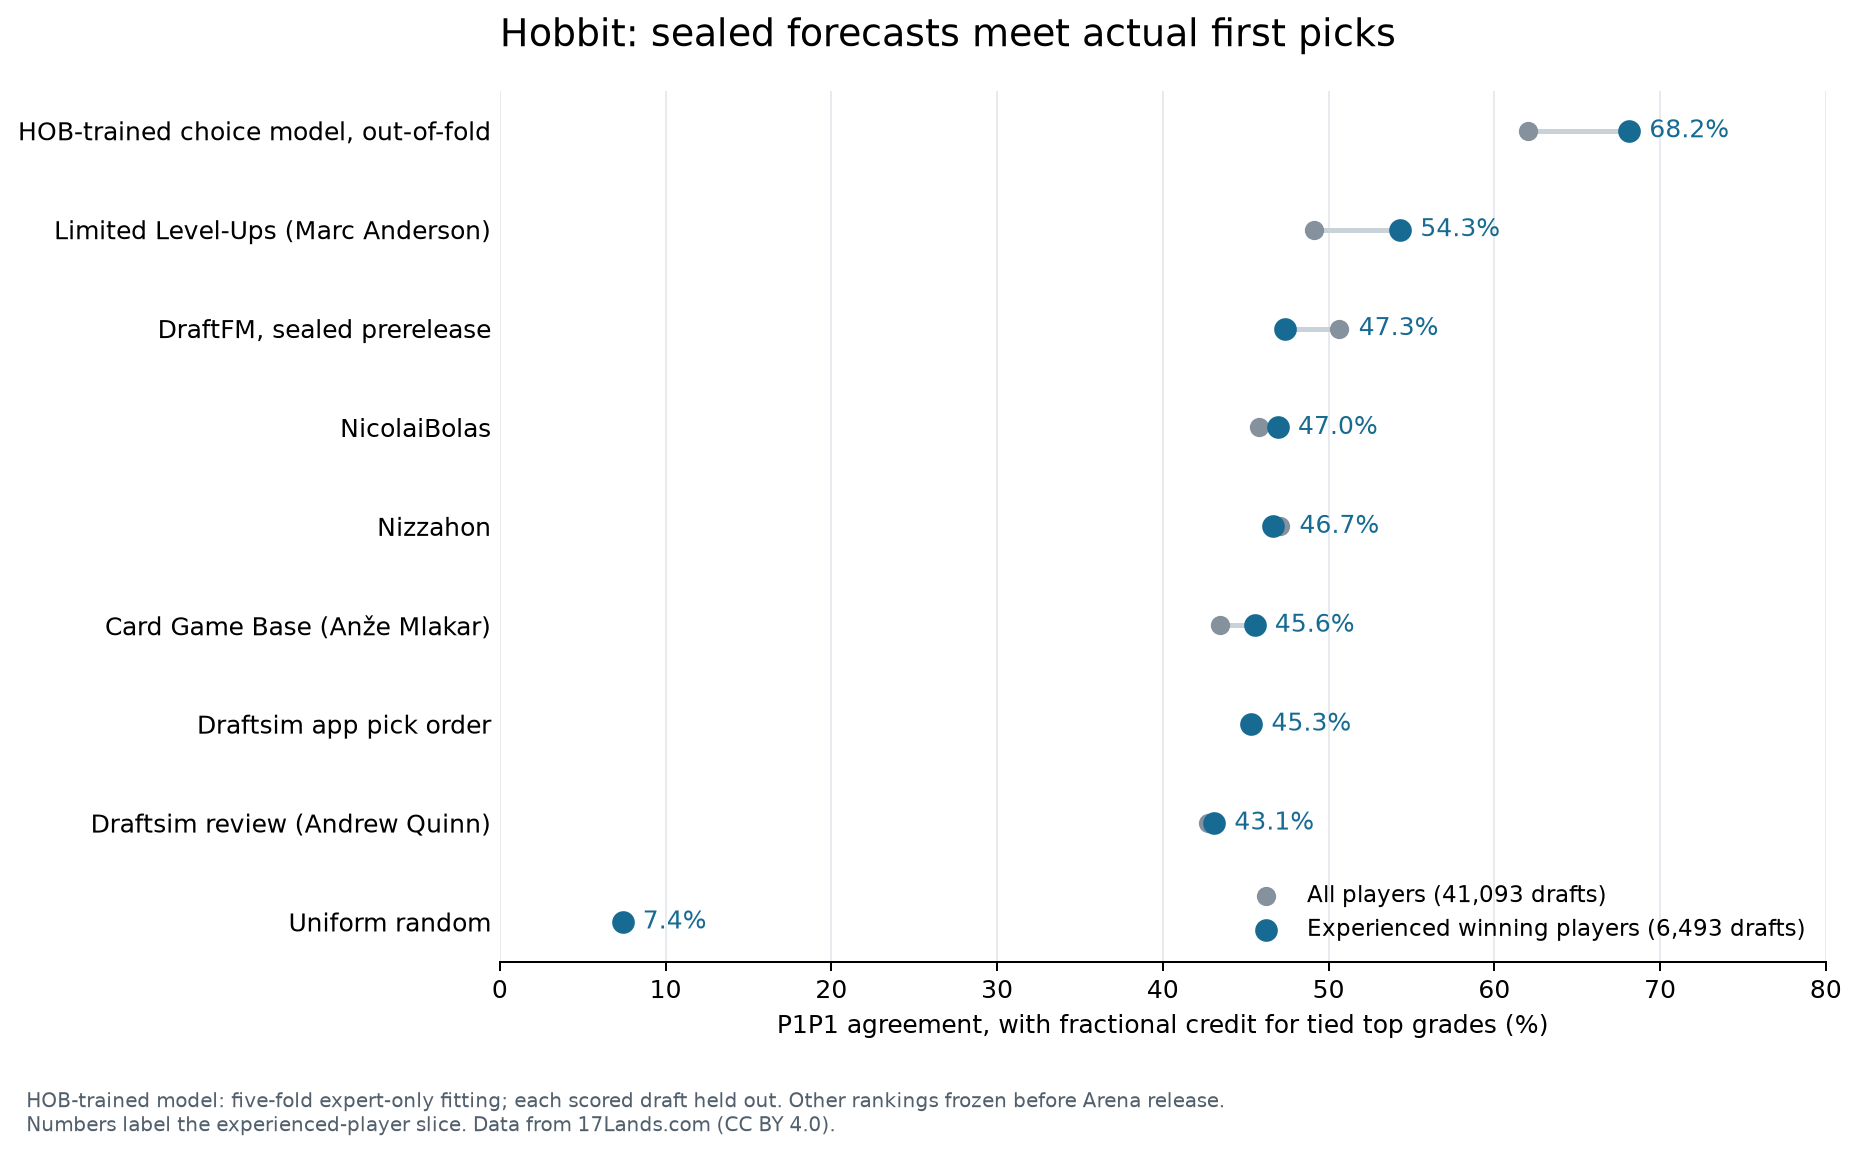
\includegraphics[width=\linewidth]{../docs/results/hob_oos_20260920/p1p1_comparison.png}
\caption{Agreement across the two populations. The plotted percentages label
the experienced-player slice; paired uncertainty is reported in
Table~\ref{tab:paired}.}
\label{fig:comparison}
\end{figure}

Coarse review grades deserve a sensitivity check. If any tied-best card
instead counted as a full success, Limited Level-Ups would reach 62.88\%,
while DraftFM would remain at 47.34\%. Fractional credit is the headline
metric, but the alternative makes its interpretation explicit. We evaluate
what the archived grades encode. We cannot recover a creator's unrecorded
preferences among equally graded cards or their complete drafting ability.

We also checked secondary outcome associations. The cached card-ratings
response contains 188 names but only 18 cards with a non-null game-in-hand
win rate and at least 200 observations, and only 52 with usable
average-taken-at values and positive pick counts. DraftFM's Spearman
correlations are $-0.232$ with game-in-hand win rate on the first subset and
$0.518$ with negative average-taken-at on the second. Those selective samples
cannot support a set-wide card-win-rate claim. The complete computed
associations are retained in the supplement, including Limited Resources.

\section{What observing HOB drafts buys}

After the initial comparison, we added a simple set-specific reference.
It learns one scalar $w_c$ for each of HOB's 188 observed non-basic cards.
For an offered pack $C_d$, its choice probabilities are
\begin{equation}
 p_w(c\mid C_d)=\frac{\exp(w_c)}{\sum_{j\in C_d}\exp(w_j)}.
\end{equation}
On training drafts $D$, it minimizes
\begin{equation}
 \sum_{d\in D}\left[\log\sum_{j\in C_d}\exp(w_j)-w_{y_d}\right]
 +\frac{1}{2}\sum_c w_c^2.
\end{equation}
These are card identities learned from HOB choices. No card text,
structured features, creator grades, game outcomes, or DraftFM warm start
enter the fitted values. This is deliberately a small conditional-choice
benchmark, not a new neural architecture.

We assign drafts to five folds using CRC32 of the draft ID modulo five.
Each fit uses experienced-player drafts from four folds and scores only
the other fold. All drafts in a scored fold are excluded from its fit,
including when we report the all-player population. The fits use
5,494--5,548 training drafts each. Fixed unit ridge regularization,
zero initialization, and L-BFGS-B optimization were specified before
computing this addendum's results; no hyperparameter search was performed.
All five fits converged, in 42--45 iterations.

The HOB-trained ranking reaches 68.15\% on the 6,493 shared experienced-player
packs. Its advantage is 20.81 points over DraftFM (95\% interval
19.47--22.09), and 13.82 points over Limited Level-Ups (12.72--14.89).
Training agreement ranges from 68.37\% to 69.27\%; those are diagnostics,
not the headline result. The headline predictions are all held out.

The gain shows that post-release choices contain useful information missing
from these prerelease rankings, even for a model with only 188 values.
It does not show that 188 parameters are generally better than DraftFM's
roughly 1.6 million. The models have different information: the fitted
reference has seen thousands of decisions from the target set. Nor is its
result a theoretical ceiling. More expressive approaches could perform
differently, and matching an observed choice remains distinct from improving
a player's results.

This addendum is exploratory: its recipe followed inspection of the first
creator comparison. Random folds mix dates, so it estimates performance on
other drafts from this release period rather than future deployment after
a particular training cutoff. Its intervals condition on fitted predictions
and omit training variance and dependence from overlapping training folds.
These qualifications leave the large observed gap intact while defining
what the experiment actually tests.

\section{Reality Fracture: put another prediction on the table}

The next set offers a chance to repeat the exercise. Wizards lists FRA's
Arena release as September 29, with tabletop prerelease beginning September
25~\cite{fra}. Using the same frozen checkpoint and feature manifest, we
scored a September 19 card snapshot on September 20. The forecast
contains 295 unique names: 285 FRA cards, including five display-only basics,
and the ten associated Special Guests. The draftable preview includes FRA
and its Special Guests, not the separate Commander product. Alternate
printings collapse to one name, using the main set and lowest numeric
collector number to select the canonical printing's features.

Table~\ref{tab:fra} gives the top ten. Six are planeswalkers, headed by
Garruk, Veiled Butcher; the first five appear in
Figure~\ref{fig:fra-cards}. Chandra, Torch of Defiance is a main-set reprint in
the snapshot (FRA 244), rather than a stray Special Guest. These names make
for a lively preview: there is plenty at the top that looks capable of
dominating a game. That is a qualitative impression, not a measured forecast
of format speed or bomb density. Our letter grades allocate fixed percentile
bands, so the number of A's cannot demonstrate that FRA has more bombs than
another expansion.

\begin{table}[htbp]
\centering\small
\input{\datadir/fra_top10.tex}
\caption{The frozen model's FRA top ten. Grades are set-relative presentation
bands; the underlying raw scores determine the order. The untested forecast
was published on September 25, after prerelease began.}\label{tab:fra}
\end{table}

\subsection{A bold ``mythic uncommon'' pick}

The more entertaining prediction is the uncommon ranking. Among all 109
FRA uncommons, DraftFM puts \emph{Terminal Criticism} first
(Table~\ref{tab:uncommons}; Figure~\ref{fig:fra-cards}). It is a two-mana
black instant whose removal is restricted to blue or red creatures and
planeswalkers, with one life
gained~\cite{terminal}. That is a conspicuously narrow card to nominate as
the set's ``mythic uncommon.'' The phrase here names the highest-ranked
uncommon in the forecast, not a new rarity or a claim about measured wins.

There is a fun connection: six of the model's own top ten cards are blue or
red creatures or planeswalkers that the spell can target. This observation
was made after inspecting the ranking. It is not evidence that the network
recognized those specific threats and promoted their answer. The frozen
export has no whole-set context encoder; its score does not explicitly
count those targets or model how often opposing decks will contain them.
A reader can reasonably suspect that the model is overvaluing cheap removal
and underpricing its restriction. That is precisely why this is a useful
prediction to preserve and revisit.

\newcommand{\fracard}[3]{%
  \begin{minipage}[t]{0.30\textwidth}
  \centering
  \includegraphics[width=0.92\linewidth]{figs/cards/fra/#1}\\[3pt]
  {\footnotesize #2\\#3\par}
  \end{minipage}}

\begin{figure}[tbp]
\centering
\fracard{garruk_veiled_butcher.jpg}{1. Garruk, Veiled Butcher}{A+}\hfill
\fracard{ajani_unrelenting.jpg}{2. Ajani Unrelenting}{A+}\hfill
\fracard{garruk_curse_breaker.jpg}{3. Garruk, Curse Breaker}{A+}

\vspace{10pt}

\fracard{ajani_resolute.jpg}{4. Ajani Resolute}{A+}\hfill
\fracard{sphinx_of_false_conclusions.jpg}{5. Sphinx of False Conclusions}{A+}\hfill
\fracard{terminal_criticism.jpg}{Uncommon \#1: Terminal Criticism}{B+}

\caption{The five highest-ranked FRA cards and the highest-ranked uncommon in
the frozen forecast. Numbers and grades come from the September 20
candidate published on September 25; these are predictions, not measured
card outcomes. Images show the canonical FRA printings in the September 19
Scryfall snapshot. Card images are
copyright Wizards of the Coast and reproduced at reduced size for scholarly
commentary; image source and hashes are recorded with the figure assets.}
\label{fig:fra-cards}
\end{figure}

\begin{table}[htbp]
\centering\small
\input{\datadir/fra_uncommons10.tex}
\caption{The top ten of all 109 FRA uncommons. This is a filter of the original
forecast, with no rescoring or regrading. The full uncommon ordering and the
295-card forecast accompany the note.}\label{tab:uncommons}
\end{table}

The preview preserves the original prediction instead of editing the bold
pick into something more conventional. Raw scores are logits, not card win
rates, and gaps between ranks do not supply uncertainty intervals. One
feature limitation is also recorded: the frozen structured keyword
vocabulary does not include Replicate, although card text still enters
through the fixed text encoder. The model and feature manifest have not
been retrained on FRA. The exact CSV and a first-pick evaluation recipe were
published on September 25 at
\url{https://github.com/brianward92/draftfm/releases/tag/fra-p1p1-2026-09-25}.
This is a public timestamp before Arena's September 29 release, but after
prerelease play began. It cannot serve as a pre-prerelease seal.

\section{From a forecast to a first-pick recommendation}


The evaluated policy can be served as a simple lookup. A player supplies
an opening pack, through card-name entry or resolved Arena card IDs. Match
all offered non-basic cards to the frozen forecast, sort them by raw score,
and present the leading choice with two or three alternatives. Show the
forecast date and make incomplete card coverage visible. If an offered
card has no score, a complete-pack recommendation is unavailable; silently
dropping it would change the choice problem.

This workflow needs no new training and no runtime neural inference.
Using the archived CSV also preserves the exact rounded scores used in
the HOB comparison. It is a practical first release for a manual pack tool
and a reference mode for an overlay. Later picks need the drafted pool and
the full contextual scorer; a static first-pick list does not provide that
context.

For presentation, rank and alternatives are sufficient. A normalized
softmax over offered raw scores can describe the model's distribution of
choices, but the present evaluation does not establish calibration of those
probabilities on an unseen set. A high percentage should not be labeled
the probability that a pick is correct, or that it will win. Rules text can
explain what a card does; it cannot by itself explain the neural network's
reasoning. A close score gap is useful to display as a close comparison,
without inventing statistical confidence.

For an application integrating these forecasts, a small versioned data
package is enough: card identities, raw scores, ranks, display grades, and
the forecast manifest. A reference pack-ranking function can verify that
its ordering matches the reported policy. The HOB evaluation and FRA preview
then provide both evidence for that policy and a concrete set of predictions
to display. Integration should preserve the scored card universe and
conditioning settings when recomputing scores; using the same weights alone
does not establish parity with an archived forecast.

\section{The next experiment}

Two follow-ups are especially concrete. First, preserve the published FRA
ranking and coverage rules, then freeze creator snapshots and the primary
experienced-player P1P1 metric before Arena outcomes arrive. Retain the all-player view and report missing
coverage. Preserve Terminal Criticism as the original uncommon nomination;
any later diagnosis should explain that prediction rather than replace it.

Second, measure how much set-specific data is needed to improve a frozen
ranking. Compare the zero-data forecast, the identity-only choice model,
and a model learning corrections to the frozen scores at fixed training
sizes, for example 500, 1,000, and 5,000 expert drafts. Use a chronological
held-out period and repeat across sets, with model selection confined to
training data. That would test whether transfer reduces the data needed
after release. It is a stronger basis for a broader study than the single
HOB fitted-model result alone. These are proposed experiments, not results
of this note.

The present contribution is the completed forecast check: a fixed
prerelease model was competitive with several saved reviews, a strong
human review did better on experienced players, and target-set observations
improved agreement substantially. The next forecast makes those limits
testable again, with a few card predictions worth arguing about along
the way.

\appendix
\section{Artifacts and reproduction}

The accompanying repository contains the analysis protocols, aggregate
tables, paired intervals, input hashes, and figure. The HOB forecast CSV
has SHA-256
\begin{quote}\footnotesize
\url{a16c34767aa382e7703f480207f8480484e29ad22bbab2142aa2195e9b9a94a9}.
\end{quote}
The FRA candidate CSV has SHA-256
\begin{quote}\footnotesize
\url{116fc528acd83843e283daa73492fa01041f167daebe92103d9f9a52617a348e}.
\end{quote}
HOB's raw snapshot and creator input hashes are recorded in
\path{docs/results/hob_oos_20260920/forecast_summary.json}; fitted-model
details are in the adjacent \code{fitted_summary.json}. The full local
analysis note, \path{docs/hob_out_of_sample_20260920.md}, provides executable
reproduction commands. The raw draft file is the frozen source of record;
later downloads need not be identical.

Independent checks reproduced all 43,650 forecast evaluations and all
held-out fitted predictions from saved weights, and verified fold
exclusions. The analysis tests cover tie handling, whole-pack coverage,
shared populations, name aliases, duplicate drafts, forecast hash checking,
the fitted objective's gradient, and training-fold exclusion. The paper
tables are generated from the saved aggregates, with source digests recorded
beside them; building the PDF does not refit a model.

Creator grades are the archived pre-Arena transcriptions described in the
original paper. Some timestamp evidence is weaker than a verified original
publication date: Draftsim's app date comes from an asset header, and
NicolaiBolas's record establishes retrieval. This supplement reports
aggregate comparisons and does not reproduce the creators' complete grade
tables. The included FRA grades are DraftFM's own outputs. Data attribution:
17Lands.com, CC BY 4.0; card identities and text from Scryfall.

\begin{thebibliography}{9}
\bibitem{draftfm} Brian Ward. \emph{DraftFM: A Foundation Model for Day-Zero
Drafting in Magic: The Gathering}. August 10, 2026.
Original manuscript: \code{paper/draftfm.tex} in
\url{https://github.com/brianward92/draftfm}.

\bibitem{seal} Brian Ward. \emph{DraftFM v1.0 sealed HOB forecast}.
August 9, 2026. \url{https://github.com/brianward92/draftfm/tree/draftfm-v1.0}.

\bibitem{lands} 17Lands. \emph{Public datasets}. HOB Premier Draft snapshot
retrieved September 19, 2026. \url{https://www.17lands.com/public_datasets}.

\bibitem{fra} Mike Turian and Jubilee Finnegan. \emph{Collecting Reality
Fracture}. Wizards of the Coast, September 8, 2026. Accessed September 20.
\url{https://magic.wizards.com/en/news/feature/collecting-reality-fracture}.

\bibitem{terminal} Scryfall. \emph{Terminal Criticism}, FRA 68.
Card record in the September 19, 2026 archived snapshot.
\url{https://scryfall.com/card/fra/68/terminal-criticism}.
\end{thebibliography}
\end{document}
